\section{Ondas I: Generalizações, Sobreposição e Ondas Estacionárias}
\subsection{Conteúdo Importante}
\subsubsection{Movimento Ondulatório}

O \textbf{movimento ondulatório} ocorre quando os elementos de massa deu um meio, tal como uma corda esticada ou a superfície de um líquido, faz movimentos oscilatórios relativamente pequenos, mas que, coletivamente, fornecem um padrão que viaja por longas distâncias. Este tipo de movimento também inclui o fenómeno do \emph{som}, onde as moléculas do ar à nossa volta fazem pequenas oscilações mas, coletivamente, causam uma perturbação que pode viajar uma longa distância.

\subsubsection{Tipos de Ondas}
Em alguns tipos de movimento ondulatório, o movimento dos elementos do meio é (para a maior parte) perpendicular ao movimento da perturbação. Isto é verdade para ondas numa corda, por exemplo. Este tipo de onda é chamada \textbf{onda transversal} e é o tipo mais fácil de visualizar.

\begin{figure}[h!]
    \centering
    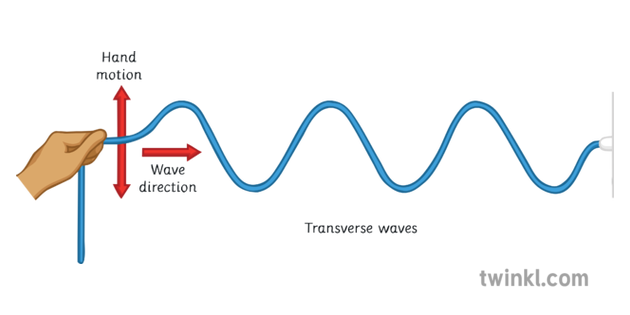
\includegraphics[width=0.5\textwidth]{11/fig/Transverse-Waves.png}
    \caption{Onda transversal.}
\end{figure}

Para outras ondas, o movimento dos elementos do meio é paralelo ao movimento da perturbação. Este tipo de onda pode ser vista quando alongamos uma mola e abanamos a sua extremidade paralelamente ao seu comprimento. Observar-se, posteriormente, regiões onde a mola está mais comprimida e esticada. Uma onda sonora viaja da mesma maneira; neste caso, as moléculas de ar têm um pequeno movimento em forma de \emph{"vai-e-volta"} que egra regiões onde o ar tem maior e menor compressão.

Uma onda viaja ao longo da direção de propagação é uma \textbf{onda longitudinal}.

\begin{figure}[h!]
    \centering
    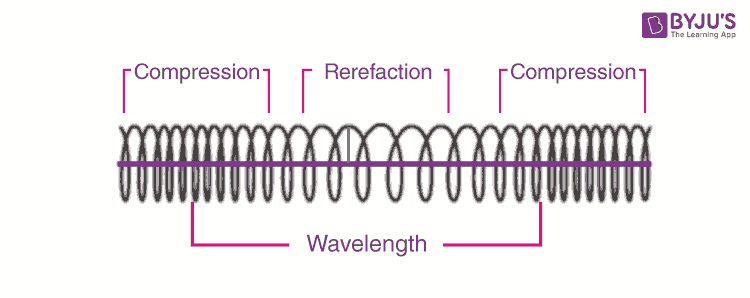
\includegraphics[width=0.5\textwidth]{11/fig/Longitudinal-Waves-1.png}
    \caption{Onda longitudinal.}
\end{figure}

\subsubsection{Descrição Matemática de uma Onda; Comprimento de Onda, Frequência e Velocidade da Onda}

No tratamento matemático dos fenómenos ondulatórios, lidaremos maioritariamente com ondas que viajam em uma dimensão. A coordenada ao longo da qual a perturbação viaja será $x$; em cada valor de $x$, o meio irá se "deslocar" de alguma maneira, e esse deslocamento será descrito pela variável $y$. Então, $y$ dependerá de $x$ e do tempo $t$ no qual se vê o deslocamento. Em geral, $y=f(x,t)$.

Se nos especializarmos no caso em que a forma da onda não muda com o tempo, mas em vez disso viaja ao longo do eixo $+x$ com uma velocidade $v$, então a onda será apenas uma função da combinação $x-vt$:

\begin{equation*}
    y=f(x-vt) \qquad \text{(Velocidade v na direção +x).}
\end{equation*}

A partir da expressão acima, segue-se que uma onda viajando na outra direção é:

\begin{equation*}
    y=f(x+vt) \qquad \text{(Velocidade v na direção -x).}
\end{equation*}

Por razões que são basicamente matemáticas, é importante estudar uma onda particular que tenha uma forma sinoidal em função de $x$. Essa onda é dada por

\begin{equation}\label{eq:onda-sin}
    y(x,t)=y_m\sin(kx\mp \omega t)
\end{equation}

Nesta equação, o sinal $-$ é utilizado para uma onda que viaje na direção $+x$; $+$ é escolhido para uma onda que viaja na direção $-x$.

Esta forma de onda representa um \emph{comboio de ondas} (infinito) em vez de um pulso. Na Equação \ref{eq:onda-sin}, $k$ é o \textbf{número de onda angular}, cuja unidade é $m^{-1}$. $\omega$ é a \textbf{frequência angular} e tem unidades $s^-1$.

A onda harmónica na Equação \ref{eq:onda-sin} é periódica no espaço e no tempo. O \textbf{comprimento de onda} $\lambda$ da onda é a distância entre repetições da forma sinusoidal da onda quando "congelamos" a onda no tempo. É possível mostrar que esse comprimento está relacionado com $k$ por:

\begin{equation}
    k=\frac{2\pi}{\lambda}
\end{equation}

O \textbf{período} $T$ da onda é o tempo entre repetições do movimento de qualquer elemento do meio. É possível mostrar que está relacionado com a frequência angular por:

\begin{equation}
    \omega=\frac{2\pi}{T}
\end{equation}

Tal como no estudo das oscilações, a \textbf{frequência} da onda tem a mesma relação com $\omega$ e $T$:

\begin{equation*}
    f=\frac{1}{T}=\frac{\omega}{2\pi}
\end{equation*}

É possível mostrar que a velocidade de tal onda (i.e. a taxa a qye a sya crusta viaja ao longo do eixo $x$) é:

\begin{equation}
    v=\frac{\omega}{k}=\lambda f
\end{equation}

Cada ponto de massa do meio move-se como uma oscilador harmónico cuja amplitude e frequência são iguais às da onda; a velocidade máxima de cada elemento é $v_{max}=y_m\omega$ e aceleração máxima de cada elemento é $y_m\omega^2$.

\subsubsection{Ondas numa Corda Esticada}
Um dos exemplos mais simples de uma onda transversal é o de ondas que viajam muma corda esticada. Pode-se mostrar que para uma corda sob uma tensão $\tau$, cuja massa por unidade de comprimento é dada por $\mu$, a velocidade das ondas é

\begin{equation}
    v=\sqrt{\frac{\tau}{\mu}}
\end{equation}

Uma caraterística importante das ondas é que \emph{transmitem energia}. A \textbf{potência média} é a taxa À qual energia mecânica passa qualquer ponto do eixo $x$. É possível mostrar que para ondas harmónicas numa corda, esta quantidade é dada por

\begin{equation}
    \bar{P}=\frac{1}{2}\mu v\omega^2y_m^2
\end{equation}

onde $\mu$ é densidade linear da corda, $v$ é a velocidade da onda e $\omega$ é a frequência angular da onda harmónica.

\subsubsection{Princípio da Sobreposição}
Uma propriedade simples de todas as ondas da natureza que estudamos é que elas se somam. Mais precisamente, se uma perturbação física de um meio gerar a onda $y_1(x,t)$ e outra perturbação gera a onda $y_2(x,t)$ então se ambos os efeitos agirem ao mesmo tempo, a onda resultante será

\begin{equation}
    y_{Tot}(x,t)=y_1(x,t)+y_2(x,t)
\end{equation}

\subsubsection{Interferência de Ondas}
Nesta e na próxima secção, são dados resultados para a sobreposição de duas ondas harmónicas que apenas diferem num aspeto.

Primeiro, consideramos duas ondas com a mesma velocidade, frequência, amplitude e direção de movimento mas que diferem por uma constante de fase. Combinaremos as duas ondas

\begin{equation}
    y_1=y_m\sin(kx-\omega t) \qquad y_2=y_m\sin(kx-\omega t + \phi)
\end{equation}

Para chegar a uma forma útil para a soma dessas duas ondas, pode-se usar a identidade trigonométrica

\begin{equation*}
    \sin\alpha+\sin\beta=2\sin\frac{1}{2}(\alpha+\beta)\cos\frac{1}{2}(\alpha-\beta)
\end{equation*}

Com isto, podemos mostrar que a onda resultante $y'(x,t)$ é:

\begin{equation}
    y'(x,t)=y_1(x,t)+y_2(x,t)=[2y_m\cos(\frac{1}{2}\phi)]\sin(kx-\omega t + \frac{1}{2}\phi)
\end{equation}

A onda resultante tem uma nova fase, mais importante, tem uma nova amplitude que depende de $y_m$ e $\phi$:

\begin{equation}
    y'_m=2y_m\cos\frac{1}{2}\phi
\end{equation}

Quando $\phi=0$, a nova amplitude é $2y_m$; as ondas dizem-se estar \textbf{completamente em fase} e que a adição é \textbf{completamente construtiva}. Um máximo da onda $y_1$ coincide com um máximo da onda $y_2$ e uma onda "maior" é o resultado.
Quando $\phi=\pi$, a nova amplitude é \emph{zero} e as ondas dizem-se estar \textbf{completamente fora de fase} e que a adição é \textbf{completamente destrutiva}. Neste caso, um máximo da onda $y_1$ coincide com um mínimo da onda $y_2$ e o resultado é o cancelamento completo.

\subsubsection{Ondas Estacionárias}
Neste capítulo, é considerado o resultado da adição de duas ondas harmónicas que têm a mesma velocidade, frequência e amplitude mas para quais as direções de propagação ($+x$ ou $-x$ são diferentes). Neste caso, as constantes de fase para cada onda são irrelevantes. Serão adicionadas as ondas:

\begin{equation}
    y_1=y_m\sin(kx-\omega t) \qquad y_2=y_m\sin(kx+\omega t)
\end{equation}

Novamente, podemos usar a identidade trigonométrica para a adição de dois $\sin$ e mostrar que a soma $y'_m(x,t)$ é:

\begin{equation}\label{eq:onda-estac}
    y'_(x,t)=y_1(x,t)+y_2(x,t)=[2y_m\cos(\omega t)]\sin(kx)
\end{equation}

A onda resultante da Equação \ref{eq:onda-estac} é uma função interessante de $x$ e $t$; no entnato não é uma onda que se propaga por não ser da forma $f(kx\mp\omega t)$. É uma função sinusoidal da coordenada $x$, multiplicada por um factor modulador $\cos(\omega t)$. Uma onda na forma da Equação \ref{eq:onda-estac} é uma \textbf{onda estacionária}.

Para a onda na Equação \ref{eq:onda-estac}, existem pontos onde não há deslocamento, i.e. aqueles onde $\sin(kx)=0$ (em que $x=\frac{n\pi}{k}$, $n$ natural). Estes pontos são os \textbf{nós} do padrão da onda estacionária.

Existem pontos para o qual o deslocamento é o máximo, nomeadamente aqueles para o qual $\sin(kx)=\pm1$ (onde $x=\frac{(2n+1)\pi}{2k}$, $n$ natural). Estes pontos são chamados os \textbf{antinós} do padrão da onda estacionária. Nós e antinós consecutivos estão separados por $\frac{\lambda}{2}$, onde $\lambda$ é o comprimento de onda das ondas originais que formaram a onda estacionária. Um nó e o antinó mais próximo estão separados por $\frac{\lambda}{4}$.

\subsubsection{Ondas Estacionárias em Cordas Sob Tensão}
Os modos de oscilação da corda são aqueles em que a corda oscila com nós em uma das extremidades e um padrão especial de nós e antinós entre eles. Esse padrão apenas existe quando a corda vibra com certas \textbf{frequências resonantes}. Para esses nós, o comprimento da corda $L$ é um múltiplo de $\frac{\lambda}{2}$:

\begin{equation*}
    L=n\frac{\lambda}{2} \qquad n=1,2,3...
\end{equation*}

que leva à fórmula das frequências resonantes:

\begin{equation}
    f_n=n\frac{v}{2L} \qquad n=1,2,3...
\end{equation}

onde $v$ é a velocidade das ondas na corda e $f_n$ é a frequência resonante do $n$-ésimo nó.